\chapter{\acs{PHP} \acs{JWT}}
\label{cha:jwt}
\sloppy

Bei der in diesem Projekt genutzten Bibliotek \glqq PHP JWT\grqq\ handelt es sich um eine objektorientierte \ac{PHP}-Klasse von \mbox{\url{firebase.com}} zur Generierung von \acl{JWT}.
\fussy
\begin{figure}[H]
	\centering
	{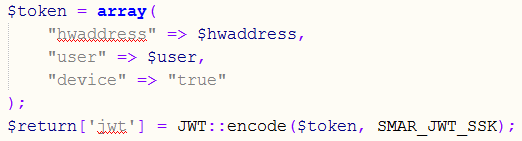
\includegraphics[scale=1.0]{Bilder/jwt_encode.png}}
	\caption{Generierung eines \acs{JWT}}
	\label{fig:jwt_encode}
\end{figure}

Abbildung \ref{fig:jwt_encode} zeigt die Generierung eines \ac{JWT}. \$token beschreibt dabei das \ac{JSON}-Objekt und enthält den Inhalt. SMAR\_JWT\_SSK ist eine in der Konfigurationsdatei festgelegte Konstante und beschreibt den Secret Server Key (geheimer Schlüssel), der nur dem Server bekannt ist, anhand dessen der Inhalt signiert wird. Dadurch wird sichergestellt, dass der \ac{JWT} bei einer weiteren Anfrage an den Server nicht durch den Client manipuliert wurde.\\

Die Dekodierung eines solchen \acl{JWT} wird in Abbildung \ref{fig:jwt_decode} beschrieben. Dabei muss SMAR\_JWT\_SSK (Secret Server Key) identisch zu dem Schlüssel sein, der zur Generierung des \ac{JWT} benutzt wurde. Sind die Schlüssel nicht identisch, wird der Token nicht dekodiert und die Funktion liefert ein leeres Ergebnis zurück.

\begin{figure}[H]
	\centering
	{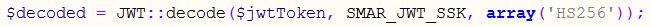
\includegraphics[scale=1.0]{Bilder/jwt_decode.png}}
	\caption{Dekodieren eines \acs{JWT}}
	\label{fig:jwt_decode}
\end{figure}

Ein \ac{JSON} Web Token setzt sich aus folgenden drei Abschnitten zusammen:\footnote{\citep[S. 289f.]{book_jwt}}
\begin{enumerate}
	\item JSON-Objekt, welches den \acs{JWT}-Header repräsentiert
	\item JSON-Objekt bestehend aus verschiedenen Name/Wert-Paaren (Claims-Set), welche die Daten des Benutzers enthält, in diesem Projekt \zB:
	\begin{itemize}
		\item die \acs{MAC}-Adresse des Gerätes und
		\item den Benutzernamen des angemeldeten Benutzers
	\end{itemize}
	\item die Signatur
\end{enumerate}
Alle drei Abschnitte sind jeweils mit BASE64-codiert und werden durch einen Punkt (.) voneinander getrennt.\\

Der \acs{JWT}-Header besteht ebenfalls aus zwei Name/Wert-Paaren und sieht in diesem Projekt wie folgt aus:
\begin{figure}[H]
	\centering
	{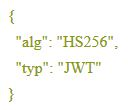
\includegraphics[scale=1.0]{Bilder/jwt_header.jpg}}
	\caption{\acs{JWT}-Header}
	\label{fig:jwt_header}
\end{figure}
Der Header beschreibt den Typ (JWT) und den verwendeten Algorithmus \shorthandoff{"} ("alg":"HS256") \shorthandon{"} zur Signierung. In \ac{SMAR} wurde der HS256-Algorithmus zur Signierung des Claims-Set verwendet. Das Claims-Set wurde somit mit einem privaten Schlüssel und SHA-256 zu einem Hash-Wert errechnet (dies ist der dritte Teil des \acs{JWT}). Die Signierung kann aufgrund des symmetrischen Signierungsalgorithmus außerdem nur mit dem selben privaten Schlüssel überprüft werden.\\
Ein \acl{JWT} stellt somit die Identität der Nachricht \bzw des \ac{JSON}-Objekt sicher und verhindert die unbemerkte Manipulation.\\

Durch den Einsatz von PHP JWT wird in \ac{SMAR} die korrekt authentifizierte Kommunikation mit der REST API - sowohl von der App, als auch von der Web Administration - sichergestellt.
Mit der Anmeldung an der Brille \bzw an der Weboberfläche wird eine Authentifizierungsanfrage an den Server (Web Administration) oder an die REST Api (\acs{VR}-Gerät) gestellt, ist die \acl{AuthN} erfolgreich, so wird ein gültiger \ac{JWT} mit Hilfe der PHP JWT-Klasse generiert. Dieser wird an die PHP-Session in der Web Administration oder an das \acs{VR}-Gerät zurückgegeben. Bei einer Anfrage an die REST Api muss dieser \acs{JWT} mitgegeben werden. Die REST Api dekodiert bei einer Anfrage zunächst den Token mit PHP JWT. Ist die Signatur gültig, wird ein JSON-Objekt zurückgegeben, ansonsten gibt es nur eine leere Antwort. Anschließend werden die Daten des JSON-Objekts mit der Datenbank verglichen, dies stellt sicher, dass die Berechtigung zur Ausführung noch vorhanden ist. Ist auch dies Erfolgreich wird die Anfrage ausgeführt. Bei einem Fehlerfall wird die Anfrage mit einer Fehlermeldung revidiert.